% Created 2024-08-20 Tue 16:13
% Intended LaTeX compiler: pdflatex
\documentclass[10pt]{article}
% =================================BASE====================================%
\usepackage[left=2cm,right=2cm,top=2cm,bottom=2cm]{geometry} % Marges
\usepackage[T1]{fontenc} % Nécessaire avec FrenchBabel
\usepackage[utf8]{inputenc} % Important pour symboles Francophones, é,à,etc
\usepackage{csquotes} % Recommandé par PDFLatex lors de la compilation. 

% Calligraphie
%\usepackage{pxfonts} % Met le texte ET les maths en Palatino + donne accès à des symboles math
%\usepackage{palatino} % Cette commande met seulement le texte en police palatino
\usepackage{lmodern} % Pour les maths? Lmodern pour les maths
\usepackage{cfr-lm}
% Use lmodern for sans-serif
\usepackage{mathrsfs} % Permet la command \mathscr (Lettres attachées genre) \mathscr(B)

% Bibliographie
\usepackage[backend=bibtex,style=apa,sorting=ynt]{biblatex}
%\usepackage[backend=biber,sorting=ynt,style=authoryear-comp]{biblatex} % N'est pas utilisé par le compilateur org-mode, mais NÉCESSAIRE. Voir le fichier init.el pour changer le style. 
\addbibresource{master-bibliography.bib}


\usepackage{amsmath, amssymb, amsthm} % Symb. math. (Mathmode+Textmode) + Beaux théorèmes.
\usepackage{mathtools,cancel,xfrac} % Utilisation de boîtes \boxed{} + \cancelto{}{}, xfrac
\usepackage{graphicx, wrapfig} % Géstion des figures.
\usepackage{hyperref} % Permettre l'utilisation d'hyperliens.
\usepackage{color} % Permettre l'utilisation des couleurs.
\usepackage{colortbl} % Color tables
\usepackage[dvipsnames]{xcolor} % Couleurs avancées.

% Physique
\usepackage{physics} % Meilleur package pour physicien. 

% Style
\usepackage{lipsum} % For fun
\usepackage{tikz} % Realisation de figures TIKZ.
\usetikzlibrary{arrows.meta,bending} % Arrow heads 
\usepackage{empheq} % Boite autour de MULTIPLE équations
\usepackage{bbding}

% Français
\usepackage[french]{babel} % Environnements en Français.

\usepackage{titling} % Donne accès à \theauthor, \thetitle, \thedate

% ==============================BASE-(END)=================================%





% ================================SETTINGS=================================%
% Pas d'indentation en début de paragraphe :
\setlength\parindent{0pt}
\setlength{\parskip}{0.15cm}

% Tableaux/tabular
% Espace vertical dans les tabular/tableaux
\renewcommand{\arraystretch}{1.2}
% Couleur des tableaux/tabular
% \rowcolors{3}{violet!5}{}

% Couleurs de hyperliens :
\definecolor{mypink}{RGB}{147, 0, 255}
\hypersetup{colorlinks, 
             filecolor=mypink,
             urlcolor=mypink, 
             citecolor=mypink, 
             linkcolor=mypink, 
             anchorcolor=mypink}


% Numéros d'équations suivent les sections :
\numberwithin{equation}{section} 

% Les « captions » sont en italique et largeur limitée
\usepackage[textfont = it]{caption} 
\captionsetup[wrapfigure]{margin=0.5cm}

% Retirer l'écriture en gras dans la table des matières
\usepackage{tocloft}
\renewcommand{\cftsecfont}{\normalfont}
\renewcommand{\cftsecpagefont}{\normalfont}

% Change bullet style
\usepackage{pifont}
\usepackage{enumitem}
%\setlist[itemize,1]{label=\ding{224}}
\setlist[itemize,1]{label=\ding{239}}
\renewcommand{\boxtimes}{\blacksquare}
% ================================SETTINGS=================================%



% ==============================NEWCOMMANDS================================%
% CQFD symbol
\renewcommand{\qedsymbol}{$\hfill\blacksquare$}

% Vecteurs de base :
\newcommand{\nvf}{\vb{\hat{n}}}
\newcommand{\evf}{\vb{\hat{e}}}
\newcommand{\ivf}{\vb{\hat{i}}}
\newcommand{\jvf}{\vb{\hat{j}}}
\newcommand{\kvf}{\vb{\hat{k}}}
\newcommand{\uu}{\vb{u}}
\newcommand{\vv}{\vb{v}}
\newcommand{\ust}{\vb{u}_{\ast}}

% Physics empty spaces 
\newcommand{\short}{\vphantom{pA}}
\newcommand{\tall}{\vphantom{pA^{x^x}_p}}
\newcommand{\grande}{\vphantom{\frac{1}{xx}}}
\newcommand{\venti}{\vphantom{\sum_x^x}}
\newcommand{\pt}{\hspace{1pt}} % One horizontal pt space

% Moyenne numérique entre deux points de grilles. 
\newcommand{\xmean}[1]{\overline{#1}^x}
\newcommand{\ymean}[1]{\overline{#1}^y}
\newcommand{\zmean}[1]{\overline{#1}^z}
\newcommand{\xymean}[1]{\overline{#1}^{xy}}

% Tilde over psi
\newcommand{\tpsi}{\tilde{\psi}}
\newcommand{\tphi}{\tilde{\phi}}

% Nota Bene env : (\ding{89})
%\newcommand{\nb}{$\boxed{\text{\footnotesize\EightStarConvex}\pt \mathfrak{N. B.}}$\hspace{4pt}}
\newcommand{\nb}{\underline{{\footnotesize\EightStarConvex}\pt $\mathfrak{N.B.}$\vphantom{p}}\hspace{3pt}}

\newcommand{\exemple}{
\parbox[center]{2.2cm}{\begin{tcolorbox}[sharp corners, rounded corners=northeast, rounded corners=southeast,
colback=Violet!2, colframe=black,
size=small, width=2cm, left=-0.25pt, bottom=-0.5pt,
arc is angular, arc=2.5mm, boxrule=0.35pt, leftrule=4pt, %bottomrule=1pt,
after={\enskip}] Exemple \end{tcolorbox}}}

\newcommand{\rad}{\text{Rad}}


\newcommand{\cqfd}{\hfill$\blacktriangleleft$}

% Define the nota bene environment
\usepackage{tcolorbox}
\newtcolorbox{notabene}{
     colback=blue!5,
     colframe=black,
     boxrule=0.5pt,
     arc=2pt,
     left=5pt,
     right=5pt,
     top=5pt,
     bottom=5pt,
}


\newcommand{\cmark}{\ding{52}}
\newcommand{\xmark}{\ding{55}}
% ==============================NEWCOMMANDS================================%



% ==============================PAGE-TITRE=================================%
% Titlepage 
\newcommand{\mytitlepage}{
\begin{titlepage}
\begin{center}
{\Huge \thesubtitle \par}
\vspace{2cm}
{\Huge \MakeUppercase{\thetitle} \par}
\vspace{2cm}
RÉALISÉ DANS LE CADRE\\ D'UN PROJET POUR \par
\vspace{2cm}
{\Huge ISMER--UQAR \par}
\vspace{2cm}
{\thedate}
\end{center}
\vfill
Rédaction \\
{\theauthor}\\
\url{charles-edouard.lizotte@uqar.ca}\\
ISMER-UQAR\\
Police d'écriture : \textbf{CMU Serif Roman}
\end{titlepage}
}
% ==============================PAGE-TITRE=================================%



% =================================ENTÊTE==================================%
\usepackage{fancyhdr}
\pagestyle{fancy}
\setlength{\headheight}{13pt}
\renewcommand{\headrulewidth}{0.025pt} % Ligne horizontale en haut

\fancyhead[R]{\textit{\thetitle}}
\fancyhead[L]{\ \thepage}
\fancyfoot[R]{\textit{\theauthor}}
\fancyfoot[L]{}
\fancyfoot[C]{} 
% =================================ENTÊTE==================================%
\author{Charles-Édouard Lizotte}
\date{28/06/2024}
\title{Rapport hebdomadaire}
\newcommand{\thesubtitle}{Contrat Été 2024}
\hypersetup{
 pdfauthor={Charles-Édouard Lizotte},
 pdftitle={Rapport hebdomadaire},
 pdfkeywords={},
 pdfsubject={},
 pdfcreator={Emacs 29.4 (Org mode 9.7.8)}, 
 pdflang={French}}
\begin{document}

\mytitlepage
\tableofcontents\newpage
\section{Les glaces dans le modèle de Elizabeth Hunke}
\label{sec:orgc67b7e8}

\subsection{Mise en contexte}
\label{sec:orgdbf7710}
La \textbf{rhéologie} est définit comme la science de la déformation des matériaux.
\Textcite{coon1974modeling} propose une rhéologie élasto-plastique pour les paquets de glace (\emph{see ice pack}).
\Textcite{hibler1979dynamic} propose une rhéologie comme un plastique visqueux non-linéaire.
Le papier de \Textcite{hunke1997elastic} présente une méthode numérique implicite pour solver les équation du model VP.
Selon \citeauthor*{hunke1997elastic}, l'enjeu vient du fait qu'il est difficile de modéliser la riche gamme de viscosités exprimé à l'intérieur d'un simple domaine de glace hétérogène.
Bref, un nombre impressionnant de rhéologies a été exploré.\bigskip

\nb Un model explicite extrapole le futur à l'aide des quantités passées tandis qu'un schéma implicite évaluerait le futur à l'aide de quantités inconnues à \(n+1\).\bigskip
\subsection{Les équations en jeu}
\label{sec:orgbe054d9}
La balance des forces par unité d'aire dans la glace est donnée par l'équation du mouvement en deux dimensions,

\begin{equation}
   \underbrace{\venti m \qty(\pdv{u_i}{t})}_\text{Évolution}
   = \underbrace{\venti\qty(\pdv{\sigma_{ij}}{x_j})}_{\substack{\text{Strenght of}\\\text{the ice}}}
   +\underbrace{\venti\ \tau_{ai}\ +\ \venti\tau_{wi}}_{\substack{\text{Contraintes}\short\\\text{Vent-Ocean}}}
   +\ \underbrace{\venti\varepsilon_{ij3} m f u_j}_\text{Coriolis}
   -\ \underbrace{\venti \qty(mg \pdv{H_o}{x_i})}_{\substack{\text{Élévation}\\\text{de l'eau}}},
\end{equation}
où \(\boldsymbol{\tau}_a = \qty(\tau_{ai},\pt\tau_{aj})\) et \(\boldsymbol{\tau}_w = \qty(\tau_{wi},\pt\tau_{wj})\) sont le vent et les contrainte de déformation.
Comme mentionné dans l'article : 
\begin{quote}
\emph{The strenght of the ice is represented by the internal stress tensor \(\sigma_{ij}\).}
\end{quote}
La masse de glace est exprimée par l'expression
\begin{equation}
   m = \rho_i\qty[cH + (1-c)h] + \rho_s\qty[cH_s (1-c)h_s].
\end{equation}

Pour ce qui est de la rhéologie, \Textcite{hibler1979dynamic} proposait une rhéologie elliptique \textbf{visco-plastique} qui relie les contraintes internes à l'intérieur de la glace (\emph{internal ice stress}) avec le dégré  d'étirement ou de déformation (\emph{rate of strain}) -- ou le \textbf{taux de changement de la déformation} pour être plus précis. 
Et donc la forme de cette rhéologie est donnée par
\begin{equation}
\label{eq:orgd8ec2a5}
   \sigma_{ij} = 2 \eta \dot{\epsilon}_{ij} + \qty(\zeta - \eta) \dot{\epsilon}_{kk} \delta_{ij} - P \cdot\delta_{ij}/2,
\end{equation}
où la variable
\begin{equation}
   \dot{\epsilon}_{ij} = \frac{1}{2} \qty(\pdv{u_i}{x_j}+\pdv{u_j}{x_i}),
\end{equation}
est un genre de jacobien.
On réécrit le \textbf{tenseur de déformation dans le domaine plastique} de manière plus évidente,
\begin{equation}
\label{eq:orgf317cd4}
   \boxed{\ \frac{1}{2\eta} \sigma_{ij} + \frac{\eta-\zeta}{4\eta\zeta} \sigma_{kk}\delta_{ij} + \frac{P}{4\zeta} \delta_{ij} = \dot{\epsilon}_{ij},\ }\hspace{1cm}\text{\textbf{Déformation plastique}}
\end{equation}
car ça va être important un peu plus loin.
Grossièrement, cette rhéologie permet au paquets de glace de diverger avec très peu de contrainte, mais résiste grandement à la compression et au cisaillement.\bigskip

Selon \Textcite{hunke1997elastic}, la pression (\(P\)) est en quelque sorte une mesure de la force de la glace qui dépend de la robustesse et de l'épaisseur de la glace.
\begin{equation}
   P = P^\ast c He \exp[-c^\ast(1-c)],
\end{equation}
où \(P^\ast\) et \(c^\ast\) sont des constantes données dans une table quelque part.
C'est pas mal semblable à la formulation de \Textcite{hibler1979dynamic}, car \(cH\) est approximativement la même chose que son \emph{equivalent ice thickness}.
La viscosité augmente avec la pression de sorte à obtenir
\begin{align}
   \zeta = \frac{P}{2\Delta}, && \eta = \frac{P}{2\Delta e^2}, && \Delta = \qty[(\dot{\epsilon}^2_{11} + \dot{\epsilon}^2_{22})(1 + e^{-2}) + 4 e^{-2}\dot{\epsilon}^2_{12} + 2 \dot{\epsilon}^2_{11}\dot{\epsilon}^2_{22}(1-e^{-2})]^{\sfrac{1}{2}}_.
\end{align}
Il semble que sans tension (\emph{strain}), la viscosité devienne infinie\ldots{} ce qui nous force à mettre des viscosités minimum et maximum.
Selon \citeauthor*{hunke1997elastic}, c'est un solution qui amène ses propres problèmes, donc on cherche de nouvelles solutions.\bigskip

On peut quand même se permettre de combiner les équations précédentes, ce qui donne un beau \emph{ice jumble d'équations},
\begin{align}
   m \pdv{u}{t} = \pdv{}{x}\qty[(\eta + \zeta)\pdv{u}{x}] &+\pdv{}{y}\qty(\eta\pdv{u}{y}) + \pdv{}{x}\qty[(\zeta-\eta)\pdv{v}{y}] + \pdv{}{y}\qty(\eta \pdv{v}{x}) - \frac{1}{2}\pdv{P}{x}\nonumber\\
     & + c'\qty[\qty(U_w-u)\cos\theta - \qty(V_w-v)\sin\theta] + \tau_{ai} + mfv - mg\pdv{H_o}{x},\\
   m \pdv{v}{t} = \pdv{}{y}\qty[(\eta + \zeta)\pdv{v}{y}] &+\pdv{}{x}\qty(\eta\pdv{v}{x}) + \pdv{}{y}\qty[(\zeta-\eta)\pdv{u}{x}] + \pdv{}{x}\qty(\eta \pdv{u}{y}) - \frac{1}{2}\pdv{P}{y}\nonumber\\
     & + c'\qty[\qty(V_w-v)\cos\theta - \qty(U_w-u)\sin\theta] + \tau_{aj} + mfu - mg\pdv{H_o}{y}.
\end{align}

Si on réorganise les termes du système d'équations précédentes, on retrouve une version simplifiée où les termes de Coriolis, les contraintes de surfaces (\emph{surface stresses}), la pression et les termes de \emph{tilt} sont sont incorporés dans une variable \(\vb{R}\), soit
\begin{equation}
\label{eq:orge0b77f3}
   m\qty(\pdv{\uu}{t}) = \eta \laplacian{\uu} + \vb{R}.
\end{equation}
C'est grossièrement l'équation qui nous permet le mieux de comprendre la nature plastique de la glace, même si c'est une équation d'onde. 
Lorsque \(\eta=0\), on obtient le cas spécial d'un fluide en cavitation -- un fluide dépourvu de viscosité.\bigskip

La condition de stabilité unidimensionelle pour une discrétisation explicite nous donnerait un pas de temps numérique de l'ordre de
\begin{equation}
   \Delta t \geq \frac{m}{2\eta} \Delta x^2.
\end{equation}
Bref, si on \emph{plug} les constantes, on voit qu'on obtient des temps de calculs beaucoup trop longs ou une très mauvaise précision.
Si on reprend l'équation précédente, mais en ajoutant une dimension élastique (Ajout de \(E\)) et un amortissement (\emph{damping}),
\begin{equation}
\label{eq:orgd09d0bf}
   m \pdv[2]{\uu}{t} =E \qty(\laplacian{\uu} + \frac{\vb{R}}{\eta}) + \text{amortissement},
\end{equation}
où \(E\) est un coefficient qui s'apparente au module de Young -- comme avec les bon vieux ressorts. 
Pour citer \Textcite{hunke1997elastic},
\begin{quote}
\emph{This equation is meant to represent, albeit very crudely, an elastic–plastic model of the sea ice in the regime where elastic waves dominate.}
\end{quote}
Cette formulation devrait converger au même état d'équilibre que \ref{eq:orge0b77f3}, tout en représentant un modèle élastique et plastique de la glace de mer où les ondes élastiques dominent.\bigskip

\nb L'équation \ref{eq:orgd09d0bf} diffère de \ref{eq:orge0b77f3} du fait qu'on a \(\qty(\sfrac{\partial^2 u}{\partial t^2})\) plutôt que \(\qty(\sfrac{\partial u}{\partial t})\), donc l'étirement n'est pas proportionnel à la déformation, mais plutôt au taux de déformation.
\subsubsection{La formulation élastique}
\label{sec:org11b6cf3}
Pour construire un modèle élastique, il faudrait séparer le tenseur de tension en deux parties, soit un domaine plastique et un domaine élastique.
La partie «plastique» a déjà été prise en compte à l'équation \ref{eq:orgf317cd4} et la partie élastique devrait être approximée par
\begin{equation}
   \frac{1}{E} \pdv{\sigma_{ij}}{t} = \dot{\epsilon}_{ij}. \hspace{1cm} \text{\textbf{Déformation élastique}}
\end{equation}

Lorsqu'on ajoute les contributions élastiques et plastiques (\ref{eq:orgf317cd4}), on obtient
\begin{equation}
\label{eq:org4919464}
   \boxed{\ \frac{1}{E} \qty(\pdv{\sigma_{ij}}{t}) + \frac{1}{2\eta}\sigma_{ij} + \qty(\frac{\eta - \zeta}{4\eta\zeta}) \sigma_{kk} \delta_{ij} + \qty(\frac{P}{4\zeta}) \delta_{ij} = \dot{\epsilon}_{ij}.\ }
\end{equation}
\subsection{Simplification du modèle EVP (pour mieux comprendre)}
\label{sec:orgd83b7e5}
On assume que
\begin{itemize}
\item Toutes les variations spatiales arrivent dans la direction \(x\).
\item Tous les coefficients sont constants, tous les forçages sont absorbés dans le terme \(\boldsymbol{\tau}\).
\item Le terme constant \(P/4\zeta\) est absorbé dans \(\sigma = \sigma_{11}\) et \(\sigma_{12}=\sigma_{22} = 0\).
\end{itemize}

Les équations résultantes sont
\begin{align}
   \frac{1}{E}\pdv{\sigma}{t} + \frac{\sigma}{\zeta} &= \pdv{u}{x}, \\
   m\pdv{u}{t} &= \pdv{\sigma}{x} + \tau,
\end{align}
où \(\zeta\) est une constante effective de viscosité comme auparavant.
Mentionnons qu'on retrouve le modèle VP (\emph{viscous plastic}) (\ref{eq:orgf317cd4}) dans la limite où \(E\rightarrow\infty\),
\begin{equation}
   m\pdv{u}{t} = \zeta\pdv[2]{u}{x} + \tau,
\end{equation}
tandis que la limite où \(\zeta\rightarrow\infty\), on retrouve le modèle purement élastique amortit, soit
\begin{equation}
   \pdv[2]{u}{t} = c_e^2\pdv[2]{u}{x} + \frac{1}{m}\pdv{1}{\tau},
\end{equation}
où \(c_e = \sqrt{\sfrac{E}{m}}\), soit la vitesse des ondes élastiques. 
\section{Présentation de Dany à l'Institut Isaac Newton}
\label{sec:org6005660}

\subsection{Mise en contexte}
\label{sec:orgeae215c}

Dans sa \href{https://www.youtube.com/watch?v=\_V7ozTp6SJM}{présentation à l'Institut Isaac Newton (2023)}, Dany décrit la dynamique de la zone marginale à l'aide de l'équation
\begin{equation}
\label{eq:orgd51e1f8}
   \rho_i h \qty(\dv{\uu}{t} + f \kvf\times\uu) = \vb{F}_i + \divergence{\boldsymbol{\sigma}},
\end{equation}
où la somme des forces est décrite comme
\begin{equation}
\label{eq:orgce99ce9}
   \vb{F}_i =
    \underbrace{\grande\boldsymbol{\tau}_g}_{\substack{\text{Gradient}\short\\\text{de surface}}}
   +\underbrace{\grande\boldsymbol{\tau}_a}_{\tall\text{Vent}}
   +\underbrace{\grande\boldsymbol{\tau}_o}_{\tall\text{Courant}}
   +\underbrace{\grande\boldsymbol{\tau}_b}_{\substack{\text{Plancher}\vphantom{A^2p}\\\text{océanique}}}
   +\underbrace{\grande\boldsymbol{\tau}_w}_{\substack{\text{Stress}\short\vphantom{A^1}\\\text{radiatif}\short\\\text{des vagues}}} .
\end{equation}
\(\bigstar\) Il faudrait préciser la provenance de l'équation \ref{eq:orgd51e1f8}, même si ça semble juste être une version modifiée de Navier-Stokes.\bigskip

Le terme \(\divergence{\sigma}\) -- définit comme étant la \textbf{rhéologie} -- est décrit à l'aide de l'équation de \textbf{déformation d'un plastique visqueux} \autocite{hunke1997elastic} (voir équation \ref{eq:orgd8ec2a5} plus haut), soit
\begin{align}
   & \divergence{\boldsymbol{\sigma}} = \pdv{\sigma_{ij}}{x_i},\\
   & \sigma_{ij} = 2\eta \pt\dot{\epsilon}_{ij} + \qty(\zeta - \eta) \dot{\epsilon}_{kk} \delta_{ij} - \frac{P}{2} \delta_{ij}.
\end{align}
où \(\eta\) et \(\zeta\) sont des viscosités (à définir).
La variable \(\dot{\epsilon}_{ij}\) est le tenseur de tension ou d'étirement (\emph{strain tensor}).\bigskip

\begin{figure}[htbp]
\centering
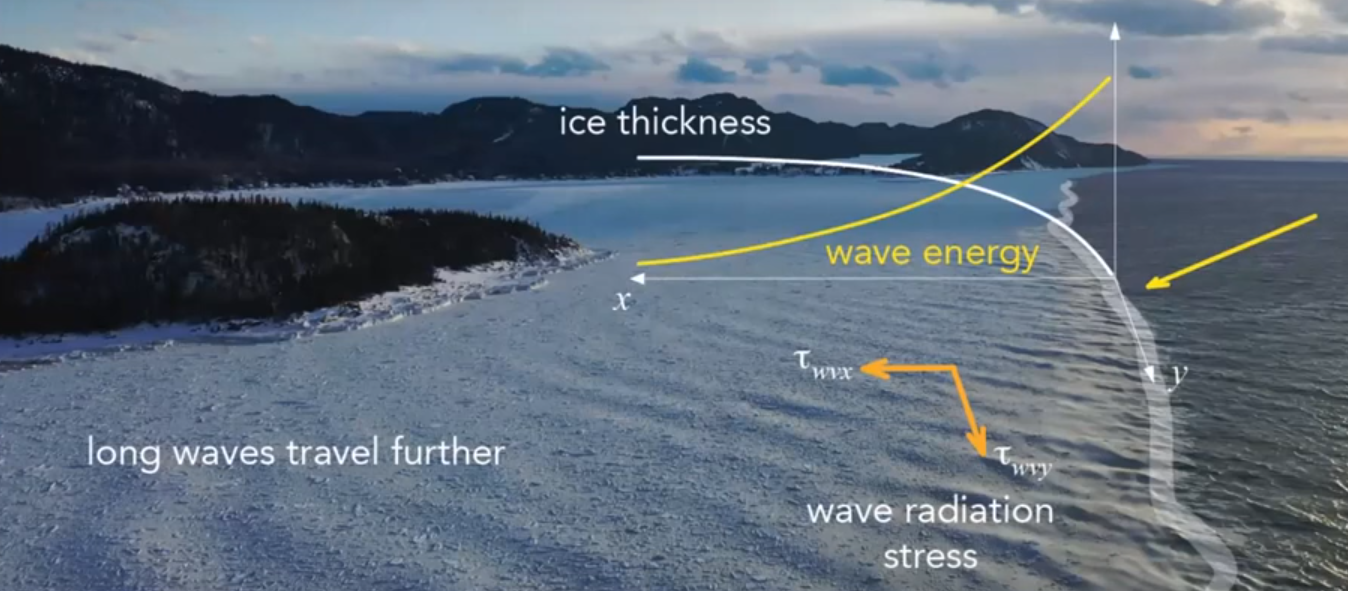
\includegraphics[width=.9\linewidth]{Figures/photos/glace-evanescente.png}
\caption{\label{fig:org66c73c5}Illustration d'un cas de figure observé à la baie du Ha-Ha.}
\end{figure}

L'onde en question se propage à la manière d'une onde évanescente dans le medium.
L'équation \ref{eq:orgd51e1f8} nous permet de visualiser deux équilibres entre l'énergie des vagues et la rhéologie, soit
\begin{equation}
   \boldsymbol{\tau}_w + \divergence{\boldsymbol{\sigma}} = 0.
\end{equation}
En posant la limite de la zone marginale à \(x=0\) (comme illustré à la figure \ref{fig:org66c73c5}) et l'arrivée des vagues avec un angle \(\phi\), on obtient deux équilibres entre les différentes forces :\bigskip

\begin{itemize}
\item \textbf{Équilibre compressif} -- Stress radiatif balance les termes de pression.
\end{itemize}
\begin{equation}
\label{eq:orgac59b44}
   \overbrace{\venti\phantom{x}\tau_{wx}\phantom{x}}^{\substack{\text{Momentum}\short\\\text{vagues-x}\short}} +\ \overbrace{\venti\frac{1}{2}\qty(\pdv{P}{x})}^{\text{Pression}\tall}\ = 0,
\end{equation}

\begin{itemize}
\item \textbf{Équilibre de cisaillement} -- Cisaillement le long du \emph{ice edge} qui balance les forces visqueuses :
\end{itemize}
\begin{equation}
   \overbrace{\venti\phantom{x}\tau_{wy}\phantom{x}}^{\substack{\text{Momentum}\short\\\text{vagues-y}\short}} +\ \overbrace{\venti\eta\qty(\pdv[\pt2]{\bar{v}}{x})}^{\text{Viscosité}\tall}\ = 0.
\end{equation}

\nb On s'attarde principalement à l'équilibre entre le transfert de momentum des vagues et la rhéologie, car le vent a peu d'impact à l'échelle désirée.
Dany élaborera son argument vers la fin de la présentation.
\subsection{Équilibre radiatif entre les vagues et la pression interne de la glace}
\label{sec:org489f68d}

Dans le milieu à l'étude, l'objectif est de représenter au moins trois types de glaces de manière générale.
On mentionne ici trois types de \emph{slush}.
Ces interactions sont modelisées à l'aide de la friction de Mohr-Coulomb. 
Dany introduit donc le \emph{ice jumble model for the compressive strenght} (voir \Textcites{uzuner1976theoretical}[][]{hopkins1999compression}[][]{dai2004wave})

\begin{itemize}
\item Friction de Mohr-Coulomb dans le plan x-z
\end{itemize}
\begin{align}
   & \sigma_x = \sigma_z\qty(\frac{1+\sin \phi}{1-\sin\phi}) \\
   & P\ = \qty(\frac{h^2}{2}) \qty(1-\frac{\rho_i}{\rho_w})(1-n)\rho_ig_e \qty(\frac{1+\sin \phi}{1-\sin\phi}) \hspace{1cm} \text{ou plutôt}\hspace{0.7cm} \boxed{\ P = K_r \cdot h^2.\ } 
\end{align}
Grossièrement, c'est proportionnel à l'épaisseur au carré (\(h^2\)) et il y a aussi un terme de \emph{porosité} (\(n\)) dans le but de représenter le fait qu'il y a des craques et des interstices dans la glace.
On définit \(K_r\) comme
\begin{equation}
   K_r =  \frac{1}{2}\qty(1-\frac{\rho_i}{\rho_w}) \qty(\frac{1+\sin \phi}{1-\sin\phi})(1-n)\rho_ig_e
\end{equation}
\bigskip

On introduit maintenant le tenseur pour la contrainte radiative des vagues  \autocite[voir][]{longuet1964radiation},
\begin{align}
   & \vb{R} = \rho g \int_0^\infty\int_0^{2\pi} F(k,\theta)
     \qty(\begin{matrix}
       c_g \cos^2 \theta + \qty(\frac{c_g}{c} - \frac{1}{2}) & c_g \cos^2 \theta \sin \theta \\
       c_g \cos^2 \theta \sin\theta & c_g \cos^2 \theta + \qty(\frac{c_g}{c} - \frac{1}{2})
     \end{matrix})
   k \cdot \dd k\pt \dd\theta\\
   & \boldsymbol{\tau}_w = - \divergence{\boldsymbol{R}} = \qty(\pdv{R_{ij}}{x_i})\cdot \evf_j
\end{align}

\textbf{À incidence normale et en eau profonde}, c'est un cas spcécial.
On se souvient que \(c_g = \sfrac{1}{2} c\), ainsi
\begin{equation}
   \boldsymbol{\tau}_w = -\frac{1}{2}\rho g \qty(\pdv{E}{x}) \ivf
\end{equation}
En partant de l'équation d'équilibre compressif (\ref{eq:orgac59b44}), on obtient une solution pour l'épaisseur de la glace, soit
\begin{equation}
   \boxed{\ h^2(x) = - \frac{\rho_w g_e E_0}{K_r}\qty(1-e^{-\alpha x}),\ }
\end{equation}
où \(E_0\) est l'énergie de l'onde incidente; \(K_r\) est un fonction de la porosité, de la friction interne et de l'angle d'incidence; puis le binôme \((1-\exp(-\alpha x))\) est la décroissance de l'énergie des vagues le long de l'axe x.
On voit apparaître un gradient dans la distribution des floes (Voir figure \ref{fig:org5b95aa9}).

\begin{figure}[htbp]
\centering
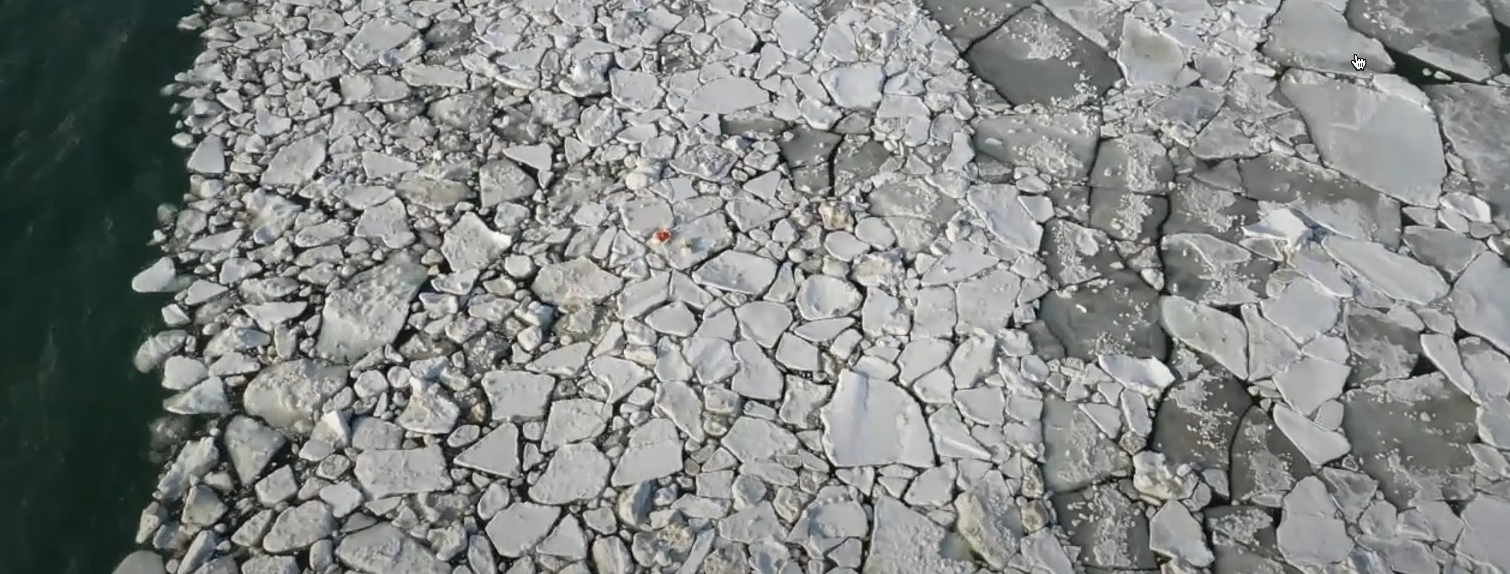
\includegraphics[width=.9\linewidth]{Figures/photos/gradient_floes.png}
\caption{\label{fig:org5b95aa9}Distribution radiale des floes dans la baie du Ha-Ha.}
\end{figure}
\subsection{Résultats empiriques pour l'équilibre radiatif}
\label{sec:org4a5c5ca}

Dans la baie du Ha-Ha, ils ont mesuré l'épaisseur du \emph{ice jumble} ainsi que l'énergie des vagues le long du transect.
De cette manière, on trouve le coefficient d'atténuation (\(\alpha\))  et la relation de dispersion de l'onde dans le milieu.
On peut même trouver l'atténuation en fonction de la fréquence de l'onde.
Le labo arrive environ à
\begin{equation}
   \alpha(\omega)  = 5.8 \times 10^{-3} \omega^{3.2}.
\end{equation}

Et on voit directement une énorme différence (2 ordres de grandeur) entre la rhéologie de Hibler et mixte
\begin{align}
   &P_{Hibler} = P^* h,\\
   &P_{MC} = K_r \cdot h^2, \hspace{1cm}\Leftarrow\hspace{1cm}\text{Pas mal meilleur}
\end{align}
où \(P^*\) est une constante.
\subsection{Équilibre de cisaillement}
\label{sec:org7dd038c}

Pas le temps pour ça.
\subsection{Conclusions}
\label{sec:orgde9400d}

\begin{itemize}
\item Dans la zone marginale stationnaire, on a isolé l'équilibre entre le transfert de momentum radiatif des vagues et la pression interne.
\item La force compressive (ou la résistance) de la glace correspod au modèle de friction de Mohr-Coulomb dans une \emph{ice jumble}.
\item La porosité est possiblement une nouvelle variable qui a besoin de recherche active.
\item La dépendance à l'épaisseur de la glace est quadratique comparativement à la version linéaire de \Textcite{hibler1979dynamic}
\end{itemize}

Aussi :
\begin{itemize}
\item Un équilibre dynamique le long du \emph{ice edge} existe est peut être utilisé pour quantifier les viscosité de cisaillement et valider les modèles.
\item La contrainte radiative des vagues peut aussi pousser le frasil sous la glace consolidée sur de longues distances, bien plus loin que le \emph{ice edge}.
\end{itemize}
\section{Résumé personnel rapide}
\label{sec:org3fd94e2}

La glace est considérées dans notre modèle comme un fluide en deux dimensions.
On prend les équations de Navier-Stokes intégrées verticalement sur l'épaisseur de la couche de glace \(h\) pour décrire son comportement dynamique, soit
\begin{equation}
\label{eq:org3e2cfc6}
    \underbrace{\venti\rho h\qty(\dv{\uu}{t} + f\kvf\times\uu)}_{\substack{\text{Accélération}\\\text{référentiel}\\\text{en rotation}}}
   =\underbrace{\venti\sum_i\vb{F}_i}_{\substack{\text{Somme}\\\text{des forces}}}
   +\underbrace{\venti\divergence{\boldsymbol{\sigma}}.}_{\substack{\text{Terme de}\\\text{Rhéologie}}}
\end{equation}
La somme des forces \(\sum_i \vb{F}_i\) est vu comme une somme de contraintes ou de forces qui agissent sur la glace.
Mentionnons que l'équation \ref{eq:org3e2cfc6} est en Pa ou en \(\text{Nm}^{-2}\).
Dans le modèle Wavewatch III, les \textbf{transferts de momentum} sont exprimés dans ces mêmes unités, ce qui pourrait rendre le couplage assez simple.
«\(h\)» est l'épaisseur moyenne de la glace dans une cellule d'aire \(A\) \autocite[voir][pour un aperçu]{dumont2022marginal}. 
Comme exprimé à l'équation \ref{eq:orgce99ce9}, ça peut représenter toutes les interactions externes à la glace, soient l'élévation du gradient de surface (\(\boldsymbol{\tau}_g\)), le vent (\(\boldsymbol{\tau}_a\)), les courants sous-jacents (\(\boldsymbol{\tau}_o\)), le contact avec le fond de l'eau (\(\boldsymbol{\tau}_b\)) ou la contrainte radiative des vagues (\(\boldsymbol{\tau}_w\)).\bigskip

Pour l'essentiel, la \textbf{rhéologie} est la manière qu'un matériau réagit aux contraintes qui lui sont infligées.
Concrétement, c'est le terme \(\divergence{\boldsymbol{\sigma}}\) qui agit comme un terme dans l'équation dynamique \ref{eq:org3e2cfc6}. 
On peut exprimer ce terme comme la divergence d'une matrice, qu'on appelle le \textbf{tenseur de contraintes} \(\boldsymbol{\sigma}\) (ou en notation matrices 2-dimensions \(\qty[\sigma_{ij}]\)).
En \textbf{deux dimensions}, les contraintes sont illustrées à la figure \ref{org5d2c2cd}.\bigskip

\begin{figure}[h]
\begin{center}
\begin{tikzpicture}
   % Étirement
   \fill[red!10]  (0,0) rectangle (1,1);
   \draw [-latex, line width = 1.5mm, orange] (-1,0.5) -- (0.2,0.5);
   \draw [-latex, line width = 1.5mm, orange] (2,0.5) -- (0.8,0.5);
   \filldraw [color=red!60,fill=red!25, thick] (0.25,0) rectangle (0.75,1);
   \draw (0.5,1.7) node[] {Compression};
   \draw[black, dotted] (0.5,-0.1) -- (0.5,1.2);
\end{tikzpicture}\hspace{2cm}
\begin{tikzpicture}
   % Compression
   \fill[blue!10] (-0.25,0) rectangle (1.25,1);
   \draw [-latex, line width = 1.5mm, orange] (0,0.5) -- (-1,0.5);
   \draw [-latex, line width = 1.5mm, orange] (1,0.5) -- (2,0.5);
   \filldraw [color=blue!60,fill=blue!15, thick] (0,0) rectangle (1,1);
   \draw (0.5,1.7) node[] {Étirement};
   \draw[black, dotted] (0.5,-0.1) -- (0.5,1.2);
\end{tikzpicture}\hspace{2cm}
\begin{tikzpicture}
   % Compression
   \fill[red!10]  (0.25,0) rectangle (1.25,1);
   \filldraw [color=orange!70,fill=orange!20, thick] (0,0) -- (0.5,1) -- (1.5,1) -- (1,0) -- (0,0);
   \draw [-latex, line width = 1.5mm, orange] (0.5,0) -- (-0.75,0);
   \draw [-latex, line width = 1.5mm, orange] (1,1) -- (2.25,1);
   \draw (0.75,1.7) node[] {Cisaillement};
   \draw[black, dotted] (0.75,-0.1) -- (0.75,1.2);
\end{tikzpicture}
\end{center}
\caption{\label{org5d2c2cd}Illustrations des différentes contraintes pouvant s'appliquer sur un élément infinitésimal en deux dimensions.}
\end{figure}

Différents matériaux réagiront différement aux contraintes, c'est pourquoi il est important de différentier les \textbf{contraintes} et la \textbf{déformation}.
La déformation sera le résultat de l'effet de la contrainte sur le matériau.
En deux dimensions, le taux de déformation (\emph{strain rate tensor}) est définit avec un tenseur (ou une matrice symmétrique) du même nom, soit
\begin{equation}
   [\dot{\epsilon}_{ij}]  = \qty[\frac{1}{2}\qty(\pdv{u_i}{x_j} + \pdv{u_j}{x_i})]
   = \begin{bmatrix}
     \sfrac{\partial u}{\partial x} & \qty(\sfrac{1}{2})\pt\pt\qty[\sfrac{\partial u}{\partial y}+\sfrac{\partial v}{\partial x}]\\
     \qty(\sfrac{1}{2})\pt\qty[\sfrac{\partial u}{\partial y}+\sfrac{\partial v}{\partial x}] & \sfrac{\partial v}{\partial y}\\
   \end{bmatrix}.
\end{equation}
de sorte que le taux de déformation est une fonction des contraintes de cisaillement
\begin{equation}
   \dot{\epsilon}_{ij} = f\qty(\sigma_{ij}),
\end{equation}
et c'est cette même fonction qui décrit comment le matériau se comporte.\bigskip

\exemple Prenons l'exemple du fluide océanique dans le modèle \emph{shallow water}.
Généralement, on ajoute une viscosité dans les modèles et ce terme possède la forme \(\nu\laplacian{\uu}\).
Ce qui signifie que
\begin{align}
   \nu\laplacian{\uu} = \divergence{\qty(\nu\gradient{\uu})},
\end{align}
et donc que la relation entre les contraintes et le taux de déformation suit la règle
\begin{align}
   \boldsymbol{\sigma}
   &= \nu\gradient{\uu} \nonumber\\
   &= \nu \begin{bmatrix}
     \pdv{u}{x} & \pdv{v}{x} \\
     \pdv{u}{y} & \pdv{v}{y} \\
   \end{bmatrix}\nonumber\\
   &= \nu\pt \mathfrak{L}
\end{align}
À partir d'ici (et selon \href{https://en.wikipedia.org/wiki/Strain-rate\_tensor}{Wikipedia}), il est possible d'utiliser la matrice \(\mathfrak{L}\) pour construire deux tenseurs, soient :
\begin{itemize}
\item le \textbf{tenseur du taux de déformation}, définit par la relation
\end{itemize}
\begin{equation}
   \mathfrak{E} = \frac{1}{2}\qty(\mathfrak{L} + \mathfrak{L}^\intercal),
\end{equation}
\begin{itemize}
\item le \textbf{tenseur du taux de rotation}, définit par la relation
\end{itemize}
\begin{equation}
   \mathfrak{W} = \frac{1}{2}\qty(\mathfrak{L} - \mathfrak{L}^\intercal),
\end{equation}
Donc, le lien entre notre tenseur de contraintes et le taux de déformation peut être exprimé par
\begin{equation}
   \mathfrak{E} = \frac{1}{2\nu}\qty(\boldsymbol{\sigma} + \boldsymbol{\sigma}^\intercal)
\end{equation}
Et donc, dans le cas de la viscosité océanique, la relation entre les éléments est donnée par
\begin{equation}
   \boxed{\ \dot{\epsilon}_{ij} = \frac{1}{2\nu}\qty(\sigma_{ij}+\sigma_{ji}),\ } 
\end{equation}
ce qui représente le rapport entre le taux de déformation est les contraintes appliquées sur notre fluide.\cqfd\bigskip

Il existe plusieurs types de rhéologies.
Dans sa \href{https://www.youtube.com/watch?v=\_V7ozTp6SJM}{présentation à l'Institut Isaac Newton (2023)}, Dany utilise principalement la formation de \Textcite{hibler1979dynamic} (eq. \ref{eq:orgd8ec2a5}), de sorte à obtenir un équilibre radiatif entre les vagues et la pression interne dans la glace.
De cette manière, il obtient une distribution d'épaisseur de glace qui satisfait les observations.\medskip

Dans l'article de \Textcite{hunke1997elastic}  l'ajout d'un terme à la rhéologie visco-plastique de \Textcite{hibler1979dynamic} (voir équation \ref{eq:orgf317cd4}) vient régler quelques problèmes associées aux cas limites.
De cette manière le modèle de glace est maintenant considéré comme visqueux, élastique et plastique (voir équation \ref{eq:org4919464}) -- d'où le sobriquet \emph{EVP model}.



\printbibliography
\end{document}
